%----------------------------------------------------------------------------------------
%	PACKAGES AND OTHER DOCUMENT CONFIGURATIONS
%----------------------------------------------------------------------------------------
\documentclass[
12pt, % Document font size
onside] % Set the document to one sided instead of two sided
{book} % Class file specifying document structure

\usepackage{graphicx} % Images package
\usepackage[a4paper,width=150mm,top=25mm,bottom=25mm,bindingoffset=6mm]{geometry} % Layout package and settings
\usepackage[backend=biber, style=apa, autocite=inline]{biblatex} % Bibliography package
\usepackage{hyperref} % Package to create hyperlinks for all cross-referenced elements
\usepackage{xcolor} % Pckage to create define colors
\usepackage{sectsty} % Package to change document styling
% ---- Packages for pseudocode ----
\usepackage{listings} 
\usepackage[ruled,vlined, linesnumbered, algochapter]{algorithm2e}
\SetKwInput{KwInput}{Input}
\SetKwInput{KwOutput}{Output}
% ---------------------------------------
\usepackage{array} % Package to write arrays
\usepackage{subcaption} % Package to create subcaptions in figures
\usepackage{physics} % Package to write math formulas

% Define colors you are planning  to use in rbg format
\definecolor{code}{gray}{0.95}
\definecolor{theme}{rgb}{0.09,0.43,0.37}
\definecolor{airforceblue}{rgb}{0.36, 0.54, 0.66}

% Pseudocode styling
\lstdefinestyle{pseudocode}{
	numbers=left,
	backgroundcolor=\color{code},
	tabsize = 2,
	numberstyle=\color{gray}
}

% Set font colors using sectsty package
\allsectionsfont{\color{theme}}

% Configure links behaviour within the document
\hypersetup{
    colorlinks=true,
    citecolor=theme,
    filecolor=black,
    linkcolor=theme,
    urlcolor= airforceblue,
}

% Biblatex configuration
\DeclareLanguageMapping{english}{english-apa}

% Add bibliography file here
\addbibresource{bibliography.bib}

% Add images folder here
\graphicspath{ {images/} }

% 
\counterwithin{figure}{section}

\lstset{style=pseudocode}
\newcommand\themebold[1]{\textcolor{theme}{\textbf{#1}}}
% Your thesis title
\title{Clustering algorithms in the touristic sector}
% Your name here
\author{Argyro Sioziou}
% Date here
\date{20 February 2020}

%----------------------------------------------------------------------------------------
%	                            DOCUMENT STARTS HERE
%----------------------------------------------------------------------------------------
\begin{document}
% Insert titlepage 
\begin{titlepage}
    \begin{center}
	% You can adjust the space here
        \vspace*{1cm}
 
        \Huge
	% Thesis title goes here
        \themebold{My thesis title}
 	% You can adjust the space here
        \vspace{0.5cm}
        \LARGE
	% If there is a thesis subtitle (e.g. case study name), it goes here
        My thesis subtitle
 
        \vspace{1.5cm}
 	% Full name goes here
        \themebold{Full Name}
	% You can adjust the space here
	\vspace{2.5cm}
 
        A thesis presented for the degree of\\
        Management Science and Technology
 	% You can adjust the space here
        \vspace{0.8cm}
	% Titlepage image
	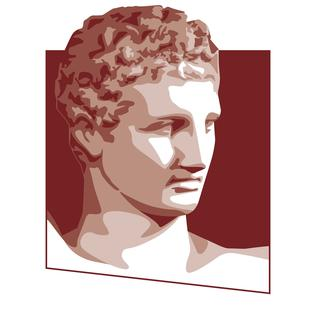
\includegraphics[width=0.4\textwidth]{titlepage_image}
	% Fill empty space
	\vfill

        \Large
        Management Science and Technology\\
        Athens University of Economics and Business\\
        Greece\\
	% Date goes here
        DD/MM/YYYY
	% You can adjust the space here
	\vspace{2.5cm}
 
    \end{center}
\end{titlepage}
% Insert abstract
\begin{center}
    % Make all titles large
    \LARGE
    % Thesis title goes here
    \themebold{My thesis title} \\
    % You can adjust the space here
     \vspace{0.5cm}
    % If there is a thesis subtitle (e.g. case study name), it goes here
    My thesis subtitle \\
    % You can adjust the space here
    \vspace{0.4cm}
    % Full name goes here
    \themebold{Full Name} \\
    % You can adjust the space here
    \vspace{1.5cm}
    \themebold{Abstract} 
\\
% You can adjust the space here
\vspace{25mm}
\end{center}
% Center paragraph
\begin{center}
Your abstract is simply a short, stand-alone summary of the thesis that others can use as an overview. It is recommended that you first finish writing your thesis and then write this part. Keep in mind to inform the reader about the problem you recognised, the purpose of your thesis, the process you are following and your conclusions.
\end{center}
\vfill
% Insert table of contents
\tableofcontents

% ---- Insert chapter titles and text ----
\chapter{INTRODUCTION}
\input{chapters/introduction}

\chapter{BACKGROUND}
\input{chapters/background}

\chapter{CASE STUDY: CLUSTER ANALYSIS ON TRAVEL AGENCY'S DATA}
\input{chapters/case}

\chapter{CONCLUSIONS}
\section{First Section}
Lorem ipsum dolor sit amet, consectetur adipiscing elit, sed do eiusmod tempor incididunt ut labore et dolore magna aliqua. Ut enim ad minim veniam, quis nostrud exercitation ullamco laboris nisi ut aliquip ex ea commodo consequat. Duis aute irure dolor in reprehenderit in voluptate velit esse cillum dolore eu fugiat nulla pariatur. Excepteur sint occaecat cupidatat non proident, sunt in culpa qui officia deserunt mollit anim id est laborum. 
\section{Second Section}
Lorem ipsum dolor sit amet, consectetur adipiscing elit, sed do eiusmod tempor incididunt ut labore et dolore magna aliqua. Ut enim ad minim veniam, quis nostrud exercitation ullamco laboris nisi ut aliquip ex ea commodo consequat. Duis aute irure dolor in reprehenderit in voluptate velit esse cillum dolore eu fugiat nulla pariatur. Excepteur sint occaecat cupidatat non proident, sunt in culpa qui officia deserunt mollit anim id est laborum. 
\section{Third Section}
Lorem ipsum dolor sit amet, consectetur adipiscing elit, sed do eiusmod tempor incididunt ut labore et dolore magna aliqua. Ut enim ad minim veniam, quis nostrud exercitation ullamco laboris nisi ut aliquip ex ea commodo consequat. Duis aute irure dolor in reprehenderit in voluptate velit esse cillum dolore eu fugiat nulla pariatur. Excepteur sint occaecat cupidatat non proident, sunt in culpa qui officia deserunt mollit anim id est laborum. 
% ------------------------------------------

% Prints bibliography page
\printbibliography
% Include bibliography to contents
\addcontentsline{toc}{section}{Bibliography}
\end{document}